\chapter{A case study of HCW disposal method selection}
\begin{flushleft}
Healthcare waste monitoring and management are crucial aspects of ensuring the safe and responsible handling of waste generated in healthcare facilities.The goal is to minimize the risks of infection, protect the environment, and ensure the safety of healthcare workers and the public. Improper management of healthcare waste can lead to the transmission of infections, jeopardizing the health of healthcare workers, waste handlers, patients, and the community. Occupational hazards, such as needlestick injuries and exposure to hazardous chemicals, are risks faced by those handling healthcare waste. The environmental impact of improper disposal can contaminate soil, water, and air, posing risks to ecosystems and public health. Inadequate waste segregation, lack of awareness and training, non-compliance with regulations, and wasteful resource usage are additional concerns. Effective healthcare waste management practices are essential to mitigate these concerns and safeguard public health while ensuring environmental sustainability.
\newline
\vspace{0.5cm}
The need for healthcare waste disposal methods is vital to address the potential risks associated with healthcare waste. Proper disposal methods are necessary to prevent the spread of infections, protect the health and safety of healthcare workers, patients, and the community.Effective healthcare waste disposal methods are essential to maintain a safe and healthy environment while mitigating potential health and environmental risks.
\section{Healthcare Waste Treatment Technologies}
\vspace{0.5cm}
There are currently four proven technologies
for achieving significant pathogen destruction, namely ‘‘incineration’’,
‘‘steam sterilization’’, ‘‘microwave’’, and ‘‘landfill’’. In this case study, we have considered these 4 alternative disposal methods.
\vspace{0.2cm}
\newline{\textbf{Incineration(A1)}: Incineration is a waste treatment process that involves the combustion of waste materials at high temperatures. It is a commonly used method for the disposal of various types of waste, including healthcare waste, hazardous waste, and municipal solid waste. It has been
claimed as the most effective means for destroying infectious
and toxic components, and for significantly reducing volume and
weight . However, the main disadvantage
of medical waste incineration is the emission of pollutants, some of them extremely toxic to the atmosphere. Pollutants are usually
emitted either in condensed or in gaseous phases. Many organic
and metallic compounds have known effects on human health
and environment}
\vspace{0.2cm}
\newline{\textbf{Steam sterilization(A2)}: The steam sterilization process involves subjecting the items to be sterilized to saturated steam at a specific temperature and pressure for a defined period of time. The high temperature and pressure within the autoclave create an environment that destroys the microorganisms by denaturing their proteins and disrupting their cellular structures. A major difficulty associated with steam
sterilization is ensuring the sufficient residence time to guarantee
pathogen destruction and the more limited capacity of most autoclaves
compared with incineration.}
\vspace{0.2cm}
\newline{\textbf{Microwave(A3)}: Large microwave irradiation medical waste treatment units include
an initial destruction phase. The waste is automatically fed
into a waste grinding device where it is shredded and sprayed with
steam to increase the moisture content of the waste. The moist
ground waste is then heated by exposure to six microwave irradiation
units over a two hour period. This process heats the waste to
greater than $90^o$ C.}
\vspace{0.2cm}
\newline{\textbf{Landfill disposal(A4)}:Sanitary land filling is the preferred method of solid waste disposal
in most situations due to its low cost, minimal environmental
impacts when designed and operated correctly, and effectiveness
in controlling health risks. Landfills must have high performance
bottom and sidewall liner systems to prevent leachate from escaping
the landfill and contaminating surrounding ground water. To
minimize water infiltrating the refuse and creating leachate, drainage
systems and cover systems must be designed and built to meet
specified performance standards}
\vspace{0.5cm}

\section{Evaluation Criteria}
These disposal methods are assessed concerning the given 6 criteria, which are:
\vspace{0.2cm}
\newline{\textbf{Cost(C1):} The estimate of annual total expenditures for HCW remediation. The financial implications associated with each disposal method, including operational costs, maintenance costs, and potential cost savings.}
\vspace{0.2cm}
\newline{\textbf{Waste Residuals(C2):} The amount and nature of residual waste generated by each disposal method, considering its impact on the environment and potential for pollution. This aspect quantifies the volume of waste impurities arising as a result of implementing a particular HCW strategy.}
\vspace{0.2cm}
\newline{\textbf{Release with health effects(C3):} The potential health risks and hazards associated with the release of contaminants or hazardous substances during the disposal process. To minimize potentially
dangerous pollutants emitted by each alternative.}
\vspace{0.2cm}
\newline{\textbf{Reliability(C4):} The dependability and effectiveness of each disposal method in terms of consistently meeting regulatory requirements and ensuring proper waste management. Long-term durability of a particular HCW treatment option.}
\vspace{0.2cm}
\newline{\textbf{Treatment effectiveness(C5):}The efficiency and effectiveness of each disposal method in treating healthcare waste to mitigate potential health and environmental risks. }
\vspace{0.2cm}
\newline{\textbf{Public Acceptance(C6):}The social acceptance and perception of the disposal method which includes public attitudes, stakeholder perceptions, and community acceptance of the method's impact on health, safety, and the environment.}
\vspace{0.3cm}
\newline
Benefiting from the literature on the assessment of health-care
disposal alternatives and discussions with the experts, it was found that out  of the above 6 criteria, C1, C2, and C3 are cost criteria and C4, C5, and C6 are benefit criteria.

\vspace{3mm}

To choose the best alternatives for HCW disposal, a committee
was created consisting of five decision-making experts $DM_1, DM_2, DM_3, DM_4$
and $DM_5$. The five experts were selected from various departments,
including a waste disposal specialist, an environmental engineer, one
professor of industrial engineering, as well as two HCW management
experts. They were interviewed several times, aiming for
attaining their judgment in regard to the weights of the six criteria
and four alternatives. The proposed
framework was well introduced, and the objective data achieved
already were provided to the experts.

\vspace{3mm}

The data collection for this study was
gathered from six hospitals in Himachal Pradesh(India) from September 2018 to
December of 2018 \cite{7}.
For the purpose of this research, a questionnaire was created
meticulously covering the assessment of HCW disposal options and
criteria. Then, for alternatives rating concerning each criterion and
the criteria weights, linguistic values were used to ask questions
from the experts. Furthermore, the linguistic terms were defined on
the basis of the survey collected by all experts. Here, we extended
the IF-TOPSIS method with AA operations for the aim of determining the optimal HCW
treatment option.

\renewcommand{\arraystretch}{1}
\begin{table}[h!]
    \centering
  
 \caption{Linguistic terms for importance rating DMs’.}
  \begin{tabular}{ p{6cm}|p{3cm}}
 \hline
 
    Ratings & IFNs \\
     \hline
   Extremely Qualified(EQ) & (1.00,0.00,0.00)\\
   Very Very Qualified(VVQ) & (0.90,0.05,0.05) \\
    Very Qualified(VQ) &  (0.70,0.20,0.10) \\
    Qualified(Q) & (0.60,0.30,0.10)\\
    Less Qualified(LS)  & (0.40,0.50,0.10)\\
   Very Less Qualified(VLQ)  &  (0.30,0.60,0.10)\\
    Extremely Less Qualified(EL)  & (0.10,0.80,0.10)  \\
    
    \hline
    \end{tabular}

\label{table:1}
\end{table}
\vspace{0.5cm}
\newline
\section{Evaluating HCW treatment alternatives}

\textbf{Step1:} As discussed above, for the evaluation of HCW treatment alternatives, 4 alternatives, 6 criteria and 5 decision making experts are considered.

\vspace{3mm}

\textbf{Step2:} Table 4.1 demonstrates the linguistic ratings that were determined by decision
experts for decision expert weight evaluation. The importance of $DM_1$ and $DM_2$ is "qualified", the importance of $DM_3$ and $DM_4$ is "very qualified" and the
importance of $DM_5$ is "very very qualified". Then, these linguistic
terms are converted into numerical values by the formula
given in eq (3.1), and the importance
weights of decision-makers are determined.
\newline
The importance weight of $DM_1$ is 0.1764
\newline
The importance weight of $DM_2$ is 0.1764
\newline
The importance weight of $DM_3$ is 0.2057
\newline
The importance weight of $DM_4$ is 0.2057
\newline
The importance weight of $DM_5$ is 0.2506


\renewcommand{\arraystretch}{1}
\begin{table}[h!]
    \centering
  \caption{Linguistic terms for rating the alternatives.}

  \begin{tabular}{ p{6cm}|p{3.3cm}}
 \hline
 
     Ratings & IFNs \\
     \hline
   Extremely poor (EP) & (0.10, 0.80, 0.10)\\
   Very poor (VP) & (0.20, 0.70, 0.10) \\
    Poor (P) &  (0.30, 0.60, 0.10) \\
    Medium poor (MP) & (0.40, 0.50, 0.10)\\
    Medium good (MG)  & (0.55, 0.40, 0.05)\\
   Good (G)  &  (0.65, 0.30, 0.05)\\
    Very good (VG)  & (0.75, 0.20, 0.05)  \\
     Extremely good (EG) & (0.90, 0.05, 0.05) \\
     \hline
     
     \end{tabular}
 
\label{table:1}
\end{table}
\renewcommand{\arraystretch}{0.7}
\begin{table}[h!]
    \centering
  
 \caption{Linguistic values of alternatives using DMs opinions.}
  \begin{tabular}{ p{1cm} p{2.5cm} p{1cm} p{1cm} p{1cm} p{1cm} p{1cm} p{1cm} }
 
 \hline
 DMs & Alternatives & \multicolumn {6} {c} {Criteria}\\
 \hline
       &    & C1 & C2 &  C3 & C4 & C5 & C6 \\
     \hline
    $DM_1$ & A1 & G & P & VG & VG & G & VG\\
 & A2 & F & F & G & P & VP & VG\\
 & A3 & MP & P & P & F & MG & P\\
 & A4 & F & P & P & F & G & P\\
$DM_2$ & A1 & VG & F & G & G & G & G\\
 &A2 & P & F & G & F & MP & G\\
 &A3 & F & P & MP & MG & F & MP\\
 &A4 & F & VP & P & F & VG & P\\
$DM_3$ & A1 & G & P & G & G & G & G\\
 &A2 & P & G & G & F & P & VG\\
 & A3 & F & P & P & F & F & P\\
 & A4 & P & F & VP & G & MG & P\\
$DM_4$ & A1 & VG & MG & G & VG & MG & MG\\
 & A2 & P & F & MG & G & P & G\\
 &A3 & F & P & P & F & F & P\\
 &A4  & F & VP & P & VG & F & F\\
$DM_5$ & A1 & VG & F & VG & G & G & VG\\
 & A2 & P & MP & F & F & P & VG\\
 &A3 & MG & P & F & F & G & MP\\
 & A4 & F & P & P & MG & MG & F\\
    \hline
 \end{tabular}

\label{table:2}
\end{table}
\newline
\vspace{0.5cm}

\textbf{Step 3:} Table 4.2 lists the linguistic ratings and the equivalent IFNs
for the HCW treatment option ratings.  Table 4.3 shows the evaluations of the options based on the
expert’s preferences.

\newline
The importance of alternatives based on criteria is
determined as linguistic terms in Table 4.3. Then, linguistic
terms are converted into numerical values using eq.(3.2) as given in Step 3.
Then, the R matrix(IF-aggregated decision matrix using DEs’
preferences) is constructed as in Table 4.4.

\vspace{3mm}


\renewcommand{\arraystretch}{1}
\begin{table}[h!]
    \centering
  
\caption{R matrix}
  \begin{tabular}{ p{1cm}  p{2cm} p{2cm} p{2cm} p{2cm} p{2cm} p{2cm} }
  \hline
   & C1 & C2 & C3 & C4 & C5 & C6 \\
 \hline
 

A1 & (0.8581, 0.0849,0.0570)&(0.4941, 0.4402,0.0657)&(0.8309, 0.1106,0.0585)&(0.8238, 0.1178,0.0584)&(0.7321, 0.2174,0.0505)&(0.8188, 0.1203,0.0609)\\
A2 & (0.3525, 0.5586,0.0889)&(0.5714, 0.3668,0.0618)&(0.6896, 0.2586,0.0518)&(0.5689, 0.3726,0.0585)&(0.3009, 0.5986,0.1005)&(0.8600, 0.0832,0.0568)\\
A3 & (0.5555, 0.3871,0.0574)&(0.3000, 0.6000,0.1000)&(0.3888, 0.5263,0.0849)&(0.5679, 0.3818,0.0503)&(0.6285, 0.3196,0.0519)&(0.3431, 0.5566,0.1003)\\
A4 & (0.5072, 0.4508,0.0421)&(0.3287, 0.5841,0.0872)&(0.2805, 0.6193,0.1002)
&(0.7252, 0.2104,0.0644)&(0.7163, 0.2218,0.0619)&(0.4278, 0.4987,0.0735)\\
  \hline
 \end{tabular}
 
\label{table:2}
\end{table}
\textbf{Step4:}  The entropy values of each IFN in the
IF aggregated decision matrix are obtained using Eqs. (3.3) and (3.4),
respectively

\vspace{3mm}

\textbf{Step5:}The weight of each criterion is calculated based on
Entropy values using Eq. (3.5). The weights of criteria are as shown
in Table 4.5.
\vspace{3mm}

\renewcommand{\arraystretch}{1}
\begin{table}[h!]
    \centering
   \caption{Weights of criteria}

  \begin{tabular}{ |p{1.5cm}|  p{1.5cm} p{1.5cm} p{1.5cm} p{1.5cm} p{1.5cm} p{1.5cm}| }
  \hline
   Criteria & C1 & C2 & C3 & C4 & C5 & C6 \\
   \hline
   Weights &0.1669 &0.1612 & 0.1667& 0.1694 &0.1670& 0.1689\\
 
    \hline
    \end{tabular}

\label{table:1}
\end{table}
\vspace{0.3cm}
\newline
\textbf{Step 6:}The PIS($A+$) and NIS($A-$) values are calculated by the equations (3.7) and (3.8). The $A+$ and $A-$ values are given in Table (4.6).

\vspace{3mm}

\textbf{Step 7:}The Separation measures for each alternative based on the
positive ideal and negative ideal solutions i.e. $S+$ and $S-$ values are calculated by the eqs. (3.9) and (3.10). The obtained values are given in Table (4.7).

 \vspace{3mm}
 
 \textbf{Step 8:} $C_i^*$ values are calculated using eq (3.11)
given in Step 8. The obtained values are given in Table (4.7).

\vspace{3mm}

\textbf{Step 9:}Taking into account the closeness values $C_i^*$, the ranks of the
alternatives are$ A4 > A3 > A2 > A1$. 

\vspace{3mm}

The results
show that A4 —landfill disposal method
is the most optimum waste disposal option and A1- Incineration is the worst alternative.

\renewcommand{\arraystretch}{1}
\begin{table}[h!]
    \centering
     \caption{Positive and negative ideal solutions}
  \begin{tabular}{ p{1.5cm} p{3cm} p{3cm}}
  \hline
  Criterion & $A+$ & $A-$\\
  \hline
  C1 & (0.3517 0.5592) & (0.8588 0.0843)\\
C2 & (0.3000 0.6000) & (0.5711 0.3672)\\
C3 & (0.2808 0.6190) & (0.8300 0.1116)\\
C4 & (0.8229 0.1187) & (0.5687 0.3805)\\
C5 & (0.7324 0.2171) & (0.3025 0.5971)\\
C6 & (0.8588 0.0843) & (0.3440 0.5557)\\

    \hline
    \end{tabular}

\label{table:1}
\end{table}
\vspace{0.3cm}

\renewcommand{\arraystretch}{1}
\begin{table}[h!]
    \centering
     \caption{Separation measures between the alternatives and final
ranking}
  \begin{tabular}{ p{2cm} p{1.5cm} p{1.5cm} p{1.5cm}}
  \hline
  Alternative & $S+$ & $S-$ & $C_i^*$\\
  \hline
  A1 & 0.3037 & 0.2731 & 0.47343\\
A2 & 0.2713 & 0.2912 & 0.51774\\
A3 & 0.2487 & 0.2671 & 0.51784\\
A4 & 0.1882 & 0.3281 & 0.63550\\
    \hline
    \end{tabular}

\label{table:1}
\end{table}
\vspace{0.3cm}




\end{flushleft}
\begin{flushleft}
    
\pagebreak
\textbf{MATLAB code}
\begin{itemize}
    

\item Aczel and Alsina Sum

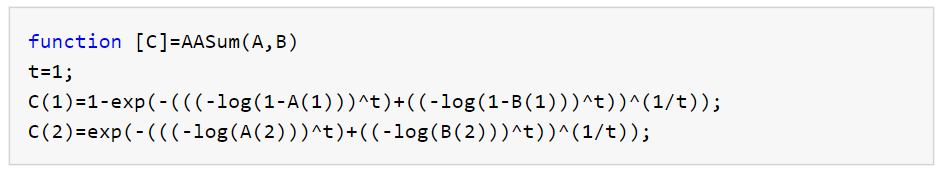
\includegraphics[width = 13cm]{config/pictures/AAsum.png}
\item Aczel and Alsina Product

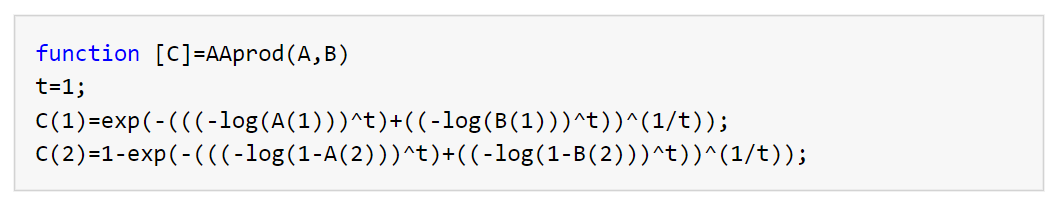
\includegraphics[width = 13cm]{config/pictures/AAProd.png}
\item Aczel and Alsina Scalar Product

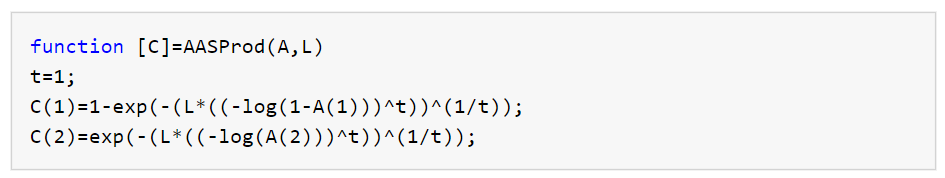
\includegraphics[width = 13cm]{config/pictures/AASprod.png}
\item Aczel and Alsina Scalar Power

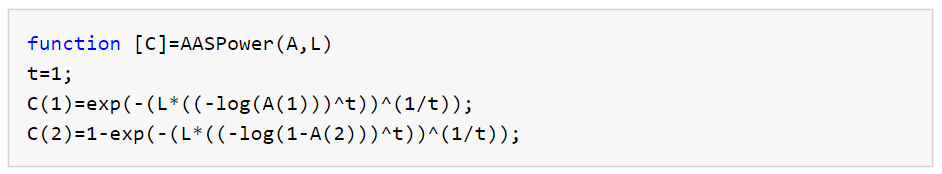
\includegraphics[width = 13cm]{config/pictures/AASpower.png}
\end{itemize}
 \item Other functions used in the MATLAB code for HCW disposal problem
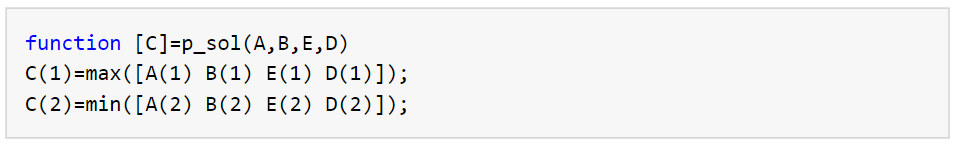
\includegraphics[width = 13cm]{config/pictures/psol.png}
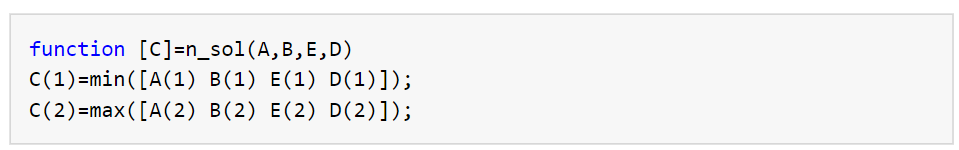
\includegraphics[width = 13cm]{config/pictures/nsol.png}
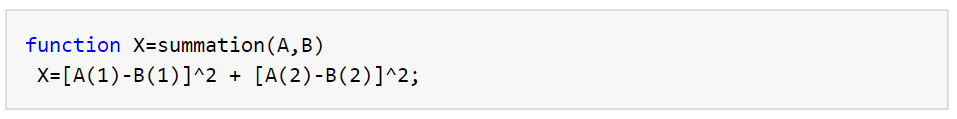
\includegraphics[width = 13cm]{config/pictures/summation.png}

 
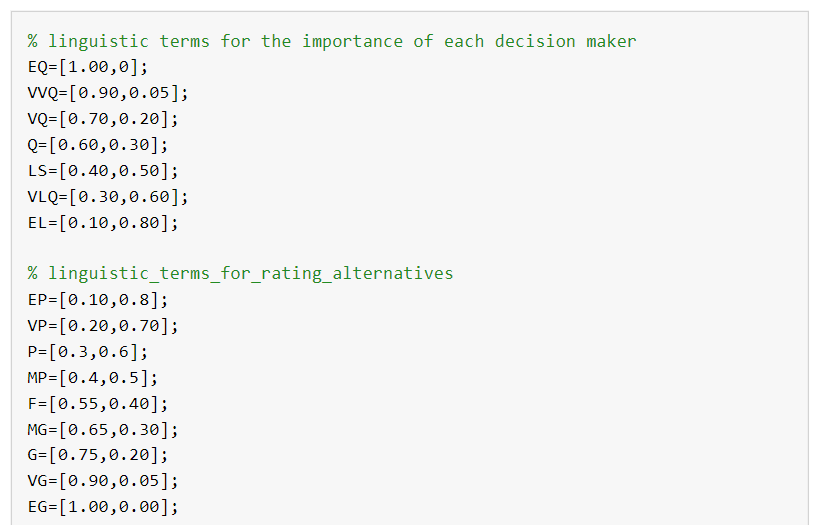
\includegraphics[width = 15cm]{config/pictures/newling1.png}
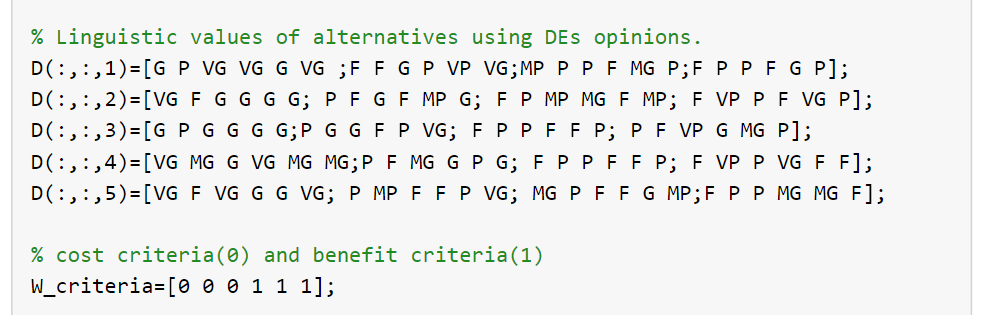
\includegraphics[width = 15cm]{config/pictures/newling2.png}
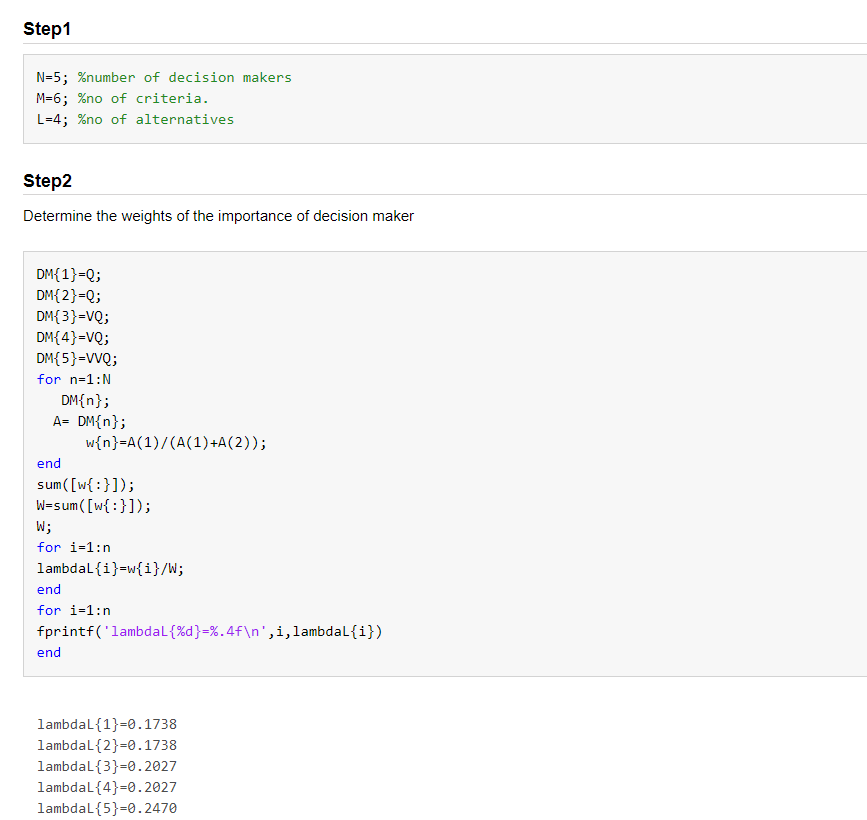
\includegraphics[width = 16cm]{config/pictures/image11.png}  
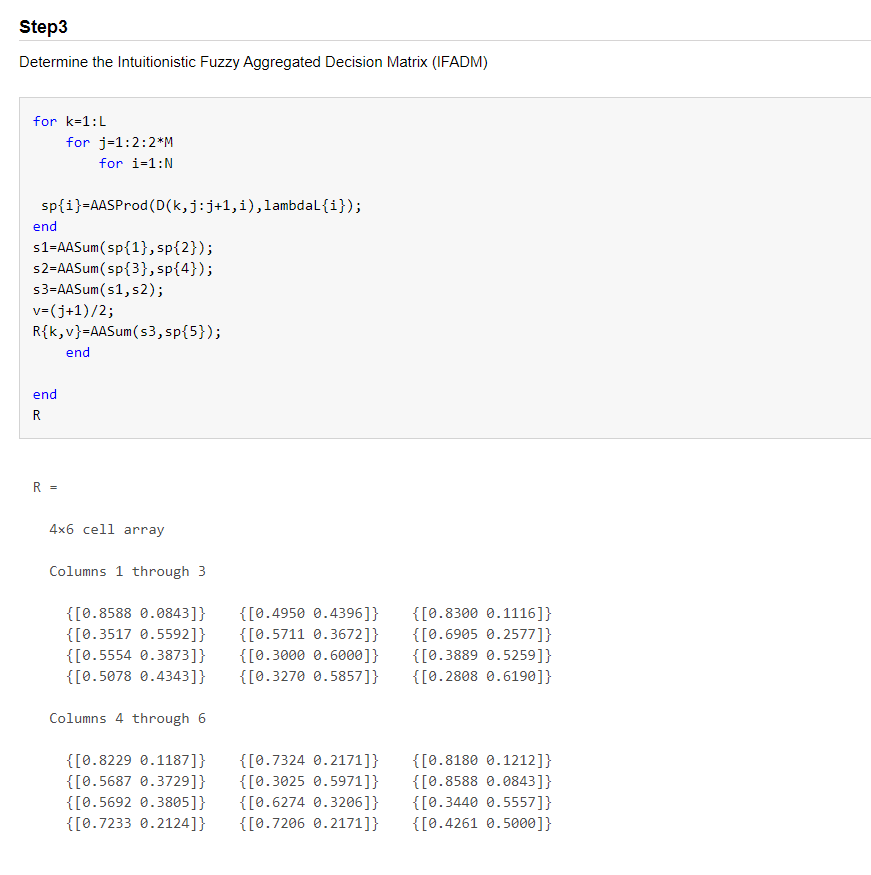
\includegraphics[width = 16cm]{config/pictures/image12.png} 
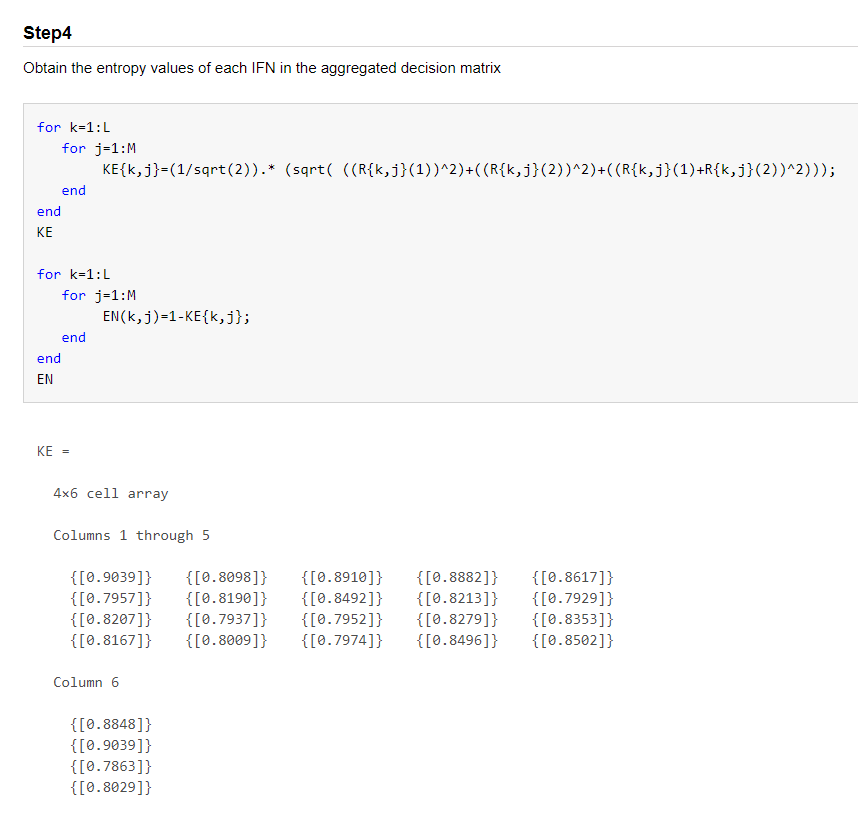
\includegraphics[width = 16cm]{config/pictures/image13.png} 
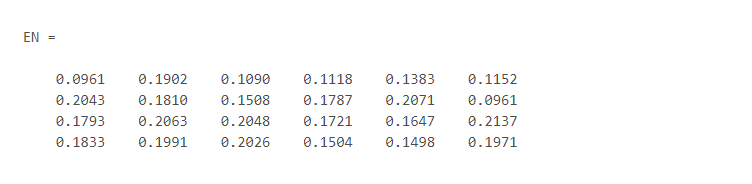
\includegraphics[width = 16cm]{config/pictures/image14.png} 
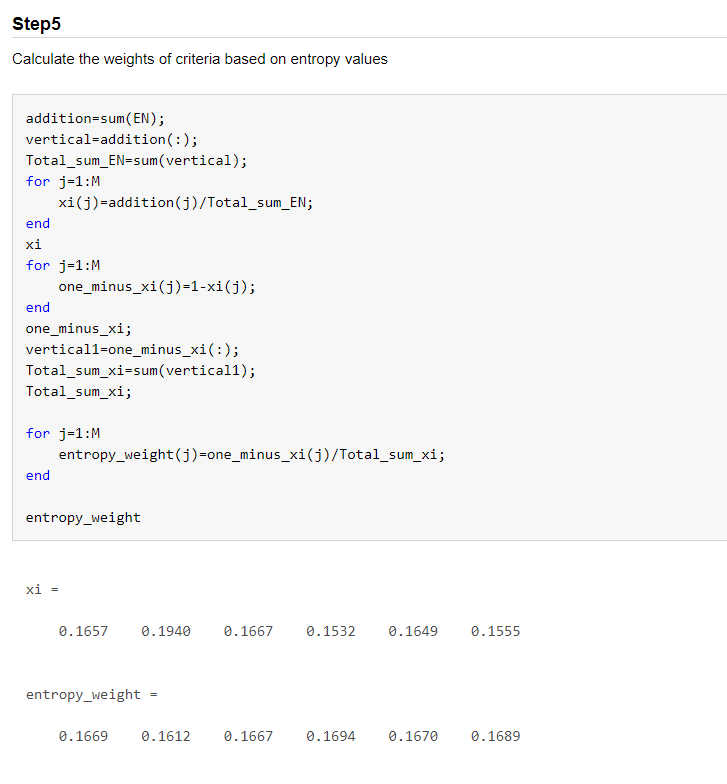
\includegraphics[width = 16cm]{config/pictures/image15.png} 
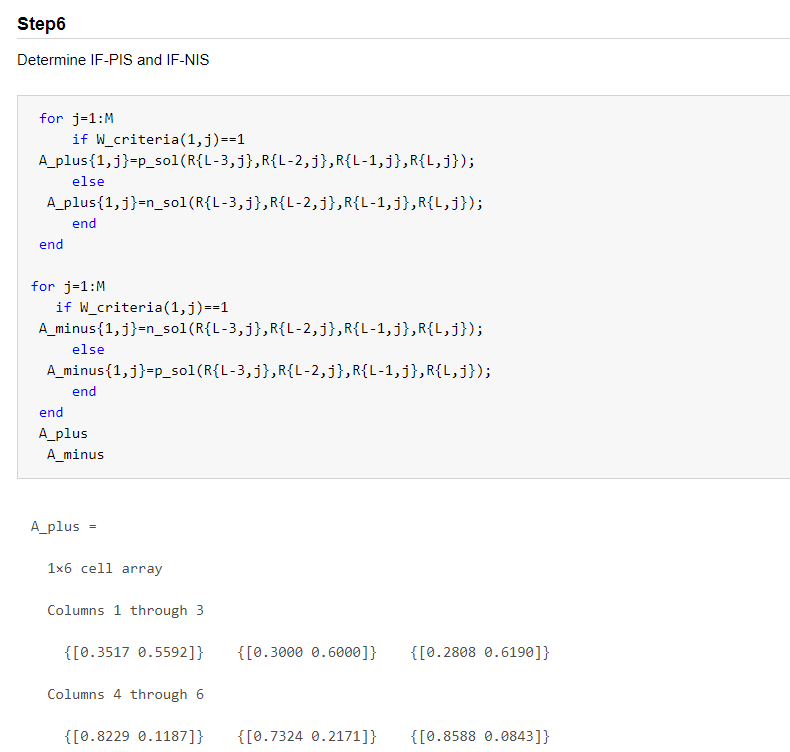
\includegraphics[width = 15cm]{config/pictures/image16.png} 
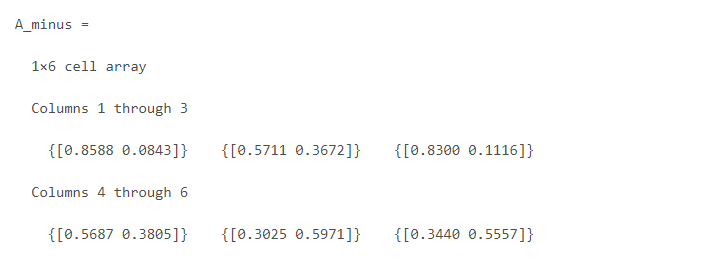
\includegraphics[width = 14cm]{config/pictures/image17.png} 
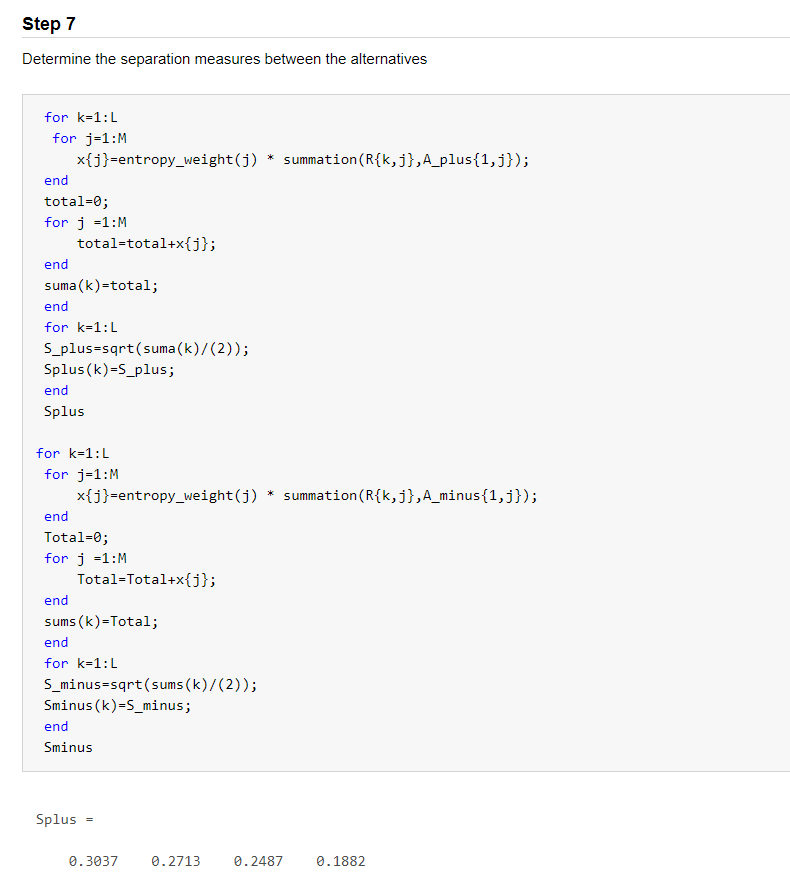
\includegraphics[width = 16cm]{config/pictures/image18.png} 
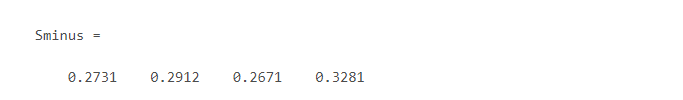
\includegraphics[width = 16cm]{config/pictures/image19.png} 
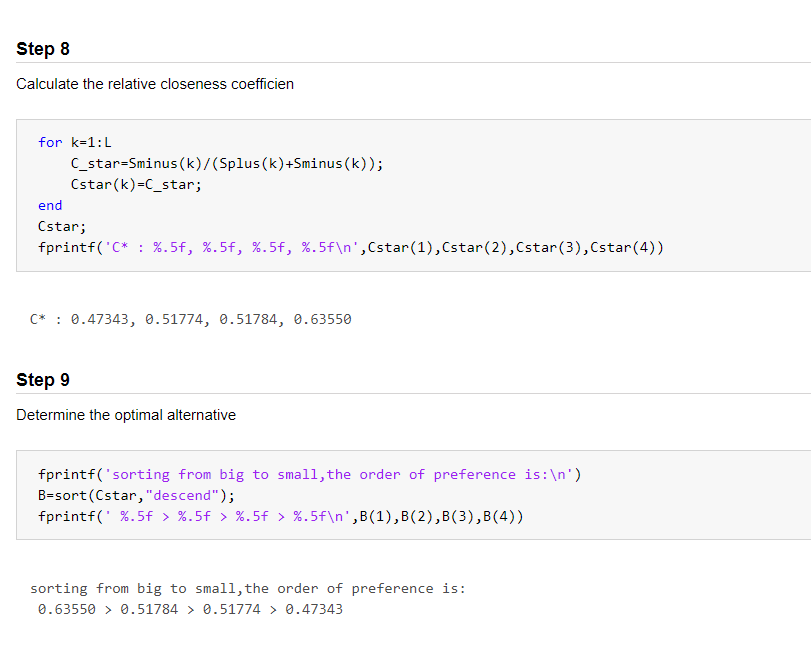
\includegraphics[width = 16cm]{config/pictures/image20.png} 
\end{flushleft}

\begin{flushleft}

 \section{Comparison of the proposed framework}

 
%\renewcommand{\arraystretch}{0.3}
\begin{table}[h!]
\resizebox{\columnwidth}{!}{% 
    \centering
   

  \begin{tabular}{ |p{3cm}|  p{3.5cm} p{3cm} p{1.5cm} p{1.5cm} p{3.5cm} p{1.5cm}| }
  \hline
   Methods & Standards & Criteria weights & MCDM process & Expert weights & Ranking order & HCW disposal option \\
   \hline
   Dursun et al. (2011a)\cite{4} & Fuzzy TOPSIS method & Assumed & Group & Assumed & $A2>A3>A4>A1$ & A2\\
   Dursun et al. (2011b)\cite{3} & Fuzzy TOPSIS based on OWA and fuzzy measure &  Weighted mean operator & Group & Considered & $A2>A3>A1>A4$ & A2\\
  Liu et al.\cite{6} & Fuzzy VIKOR method  & Triangular fuzzy
numbers & Group & Considered & $A2>A3>A1>A4$ & A2\\
A.R Mishra et al.\cite{7} & Intuitionistic fuzzy EDAS method  &  divergence
measure & Group & Considered & $A2>A4>A3>A1$ & A2\\
Proposed method & Intuitionistic fuzzy TOPSIS method  &  Entropy Method & Group & Considered & $A4>A3>A2>A1$ & A4\\

 
    \hline
    \end{tabular}%
}
\caption{Comparative analysis of alternatives ranking with diverse existing approaches.}
\label{table:1}
\end{table}
 
 \pagebreak
 Now, we observe that the framework proposed here has
considerable similarities with existing methods. The IF-TOPSIS
method is found efficient to tackle the qualitative and quantitative
MCDM problems, particularly in cases where there are several
conflicting criteria.
In this section, we illustrate a comparison of the proposed
approach with further MCDM methods based on various
vital parameters utilized in the process of MCDM (see Table 4.8).
To retain homogeneity in the method-based comparison, we consider the approaches
viz., fuzzy TOPSIS \cite{4}, fuzzy TOPSIS
with OWA and fuzzy measure \cite{3},Intuitionistic fuzzy EDAS method\cite{7}, fuzzy VIKOR
\cite{6} and proposed methods.
\vspace{0.3cm}
\newline
The list of parameters shows that the developed method is
definitely, a new contribution as it integrates all major parameters
of the MCDM process in comparison with existing literature on
methods to solve MCDM problems under uncertain environments.
\vspace{0.3cm}
\newline
From Table 4.8, we observe that the comparison of the rankings obtained from different decision-making approaches reveals some variations in the prioritization of alternative healthcare waste disposal methods. While there is consistency in the rankings of alternatives A2 and A3 across all approaches, the rankings of alternatives A1 and A4 differ.

\vspace{3mm}

Our approach (IF-TOPSIS with Aczel-Alsina operations and entropy measure) ranks alternative A4 as the highest priority, indicating its suitability as the optimal healthcare waste disposal method. On the other hand, alternative A1 is ranked lower in our approach.

\vspace{3mm}

The findings from Dursan et al.'s (2011a and 2011b) studies show a similar ranking pattern, with alternative A2 receiving the highest priority. However, there is a discrepancy in the rankings of alternatives A1 and A4.

\vspace{3mm}

Similarly, Liu et al.'s fuzzy VIKOR method also ranks alternative A2 as the most favorable, with differences in the rankings of alternatives A1 and A4.

\vspace{3mm}

AR Mishra et al.'s IF-EDAS approach yields a different ranking order, with alternative A2 still ranked the highest, but alternative A4 ranked second, followed by alternative A3 and then A1.

\vspace{3mm}

Based on this comparison, it is evident that the choice of decision-making approach can influence the rankings of alternatives. The variations in rankings highlight the importance of carefully selecting an appropriate decision-making method that aligns with the objectives, criteria, and preferences of the healthcare waste management context.

\vspace{0.3cm}
\newline
Among these four options, the decision-making implications
of landfill disposal are given by (a) it shows better
performance on social, environmental and resource aspects with
minimum operating costs. (b) Some modern landfills have implemented technology to capture and utilize the methane gas produced by decomposing waste. Methane can be used as a source of renewable energy, reducing the reliance on non-renewable energy sources.
\vspace{0.3cm}
\newline
The outcomes of the developed IF-TOPSIS framework are
compared with the results of  Dursun et al. (2011b)\cite{3}. These two
studies evaluate the HCW disposal options. In  Dursun et al. (2011a)\cite{4},
the concept of fuzzy sets was implemented to portray the experts’
opinion, while we employ the concept of IFSs to describe the experts’
opinion. The theory of fuzzy set permits the decision experts
to characterize the uncertainty using a crisp value, while the theory
of IFS permits the decision experts to signify the uncertainty using
Membership Degree, Non-Membership Degree, and hesitancy degrees, so the IFSs are more capable than
FSs. The developed framework not only evaluates the significant
degrees of considered factors but also tackles the ambiguity and
fuzziness arises through the HCW disposal assessment framework
in emerging economies.
\end{flushleft}
